\documentclass[aspectratio=169, table]{beamer}

\usepackage[utf8]{inputenc}
\usepackage{listings} 

\usetheme{Pradita}

\subtitle{MTI104 - IT Services}

\title{Session-02:\\\LARGE{ITIL 101: Concepts and\\Core Foundation}}
\date[Serial]{\scriptsize {PRU/SPMI/FR-BM-18/0222}}
\author[Pradita]{\small{\textbf{Alfa Yohannis}}}

\begin{document}

\frame{\titlepage}

\begin{frame}
	\frametitle{Introduction}
	\begin{itemize}
		\item Starts with Chapter 2, insight into DevOps.
		\item Avoids comparing ITIL concepts with previous versions.
		\item Focus on service management concepts.
		\item Covers value, outcomes, costs, and risks.
		\item Discusses utility and warranty in service relationships.
		\item Exam tips provided throughout.
	\end{itemize}
\end{frame}

\begin{frame}
	\frametitle{Service Management Overview}
	\begin{itemize}
		\item Importance of service-related options.
		\item Value of a brand linked to its services.
		\item Role of service provider in maintaining motion.
		\item Service management spans various specializations.
	\end{itemize}
\end{frame}

\begin{frame}
	\frametitle{ITIL Definition of Service Management}
	\begin{itemize}
		\item Specialized organizational capabilities for value creation.
		\item Importance of technical maturity and experience.
		\item Leadership in service management.
		\item Connection to product management.
		\item Product and service success interlinked.
	\end{itemize}
\end{frame}

\begin{frame}
	\frametitle{Products and Services in ITIL}
	\begin{itemize}
		\item Blurring lines between products and services.
		\item Example: MS Office vs. Office 365.
		\item Services drive outcomes for customers.
		\item Strategy for product management essential.
		\item ITIL focuses on both, with emphasis on services.
	\end{itemize}
\end{frame}

\begin{frame}
	\frametitle{ITIL Definition of a Product}
	\begin{itemize}
		\item Configuration of an organization's resources for value.
		\item Resources can be people, processes, products.
		\item Different ways to offer products: sale, lease, subscription.
		\item Aim to provide value through organizational resources.
	\end{itemize}
\end{frame}

\begin{frame}
	\frametitle{ITIL Definition of a Service}
	\begin{itemize}
		\item Enabling value co-creation for desired outcomes.
		\item Service provider manages risks and costs.
		\item Active customer involvement in value creation.
		\item Example: Benefits of Office 365 vs. traditional products.
	\end{itemize}
\end{frame}

\begin{frame}
	\frametitle{Organization in Service Management}
	\begin{itemize}
		\item Value creation requires collaboration.
		\item ITIL definition of an organization.
		\item Organization roles: Service provider and consumer.
		\item Example: Microsoft and Verizon mutual relationship.
	\end{itemize}
\end{frame}

\begin{frame}{Service Provider and Consumer}
	 \frametitle{Service provider and Consumer}
\begin{center}
	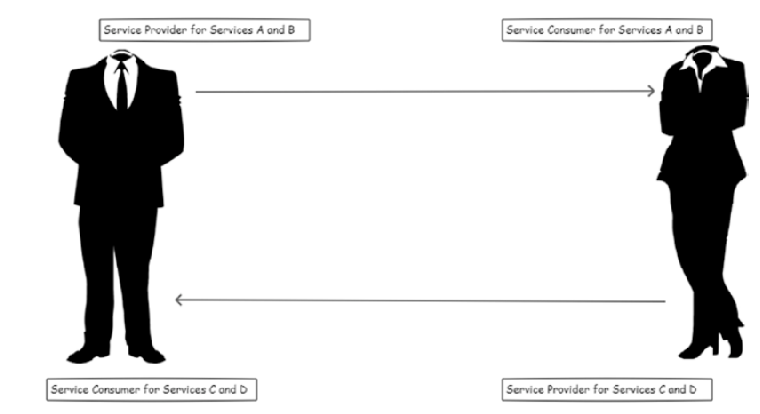
\includegraphics[width=0.6\linewidth]{images/image-01.png}
\end{center}
\end{frame}

\begin{frame}
	\frametitle{People Roles in ITIL}
	\begin{itemize}
		\item Customer, sponsor, user roles.
		\item ITIL definition of a customer.
		\item ITIL definition of a sponsor.
		\item ITIL definition of a user.
		\item Example: Multinational company purchasing laptops.
	\end{itemize}
\end{frame}

\begin{frame}
	\frametitle{Defining Value in IT Services}
	\begin{itemize}
		\item Value is perceived by the customer.
		\item Components of value: outcomes and preferences.
		\item ITIL definition of value.
		\item Importance of co-creating value.
		\item Example: Nokia and Microsoft collaboration.
	\end{itemize}
\end{frame}

\begin{frame}{Elements of value}
	 \frametitle{Elements of value}
\begin{center}
	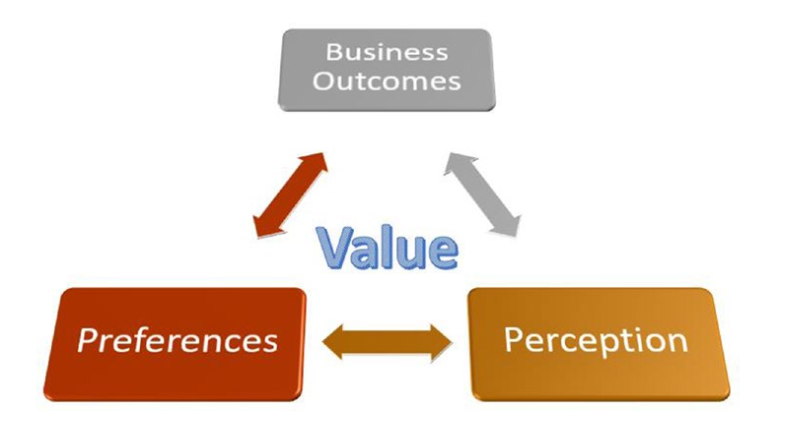
\includegraphics[width=0.8\linewidth]{images/image-02.png}
\end{center}
\end{frame}

\begin{frame}
	\frametitle{Outcomes}
	\begin{itemize}
		\item Value is co-created between the service provider and the customer.
		\item Value is highly subjective; perceptions vary between customers.
		\item Co-creating services tailors them to customer needs.
		\item ITIL Definition of Output: Tangible or intangible deliverable of an activity.
		\item ITIL Definition of Outcome: A result for a stakeholder enabled by one or more outputs.
		\item Customers judge based on outcomes, not just outputs.
		\item Objectives achieved through service are more important than outputs.
	\end{itemize}
\end{frame}

\begin{frame}
	\frametitle{Outcome vs. Output}
	\begin{itemize}
		\item Example: Netflix provides entertainment through on-demand videos.
		\item Outputs: Movies, TV shows, and documentaries.
		\item Outcomes: Customer entertainment, bonding with family.
		\item Outputs are tangible; outcomes are intangible.
		\item Outcomes depend on customer taste and perception.
		\item Services facilitate outcomes through one or more outputs.
		\item Metrics should focus on outcomes, not just outputs.
	\end{itemize}
\end{frame}

\begin{frame}
	\frametitle{Costs in ITIL}
	\begin{itemize}
		\item Costs pertain to financial transactions between consumer and provider.
		\item ITIL Definition of Costs: Money spent on an activity or resource.
		\item People costs are a significant part of service costs.
		\item Costs are calculated based on FTE (Full Time Effort).
		\item Direct costs: Imposed directly on the customer (e.g., service price).
		\item Indirect costs: Infrastructure, resources, etc., not directly charged.
		\item Service costs must be competitive and justified to consumers.
	\end{itemize}
\end{frame}

\begin{frame}
	\frametitle{Risk Management in IT Services}
	\begin{itemize}
		\item Risks are inherent in every business, including IT services.
		\item ITIL Definition of Risk: A possible event causing harm or loss.
		\item Risks can be borne by providers or consumers.
		\item Example: Uber reduces driving risks but may face connectivity issues.
		\item Service providers and consumers collaborate to manage risks.
		\item Requirements definition includes identifying and managing risks.
		\item Trust between provider and consumer is key in risk mitigation.
	\end{itemize}
\end{frame}

\begin{frame}
	\frametitle{Risk Mitigation Strategies}
	\begin{itemize}
		\item Risk Avoidance: Remove or negate the risk.
		\item Risk Transfer: Shift the risk to another party (e.g., insurance).
		\item Risk Mitigation: Counter the risk when it materializes.
		\item Risk Acceptance: Accept and prepare to deal with the risk.
		\item Example: Avoiding infrastructure uncertainties by canceling work from home.
		\item Example: Transferring car rental risks to an insurance company.
		\item Example: Mitigating server crashes with load balancing or failover mechanisms.
	\end{itemize}
\end{frame}

\begin{frame}
	\frametitle{Utility and Warranty}
	\begin{itemize}
		\item Value is created if a service is fit for purpose and fit for use.
		\item Fit for Purpose: Service meets all functional requirements.
		\item Fit for Use: Service is usable and capable of achieving outcomes.
		\item Utility of a Service: Functionality meeting a particular need.
		\item Performance Supported: Service must improve business outcomes.
		\item Constraints Removed: Service should eliminate barriers.
		\item Value creation requires both fit for purpose and fit for use.
	\end{itemize}
\end{frame}

\begin{frame}
	\frametitle{Warranty of a Service}
	\begin{itemize}
		\item ITIL Definition of Warranty: Assurance that a service meets agreed requirements.
		\item Four parts of Warranty:
		\begin{itemize}
			\item Service availability
			\item Sufficient capacity
			\item Service continuity
			\item Service security
		\end{itemize}
		\item All four criteria must be met for a service to be fit for use.
		\item Value is created when both utility and warranty conditions are satisfied.
	\end{itemize}
\end{frame}

\begin{frame}
	\frametitle{Criteria for a Service to be Fit for Use}
	\begin{itemize}
		\item Table 3-3 provides the criteria for ensuring that the service is fit for use.
		\item It is not complete for all permutations and combinations.
		\item The AND gate provides a FALSE output whenever any of the inputs are FALSE.
		\item Available capacity and continuity are important factors.
		\item Security is also a critical factor.
		\item Without these, the service is not fit for use.
		\item Service assessments consider utility, warranty, and risks.
	\end{itemize}
\end{frame}

\begin{frame}
	\frametitle{Examples of Criteria}
	\begin{itemize}
		\item Available Enough? 
		\item Scenario: No mobile coverage in a resort despite claims of good service.
		\item Capacity Enough? 
		\item Scenario: Unable to make a call due to overloaded network.
		\item Continuous Enough? 
		\item Scenario: Frequent call drops during an important interview.
		\item Secure Enough? 
		\item Scenario: Private conversation accessible over the cloud.
	\end{itemize}
\end{frame}

\begin{frame}
	\frametitle{Summary of Criteria}
	\begin{itemize}
		\item Service must be available, have sufficient capacity.
		\item Service must be continuous and secure.
		\item Any missing element devalues the service.
		\item Example: Cell phone service not fit for use without these.
		\item Assessments include service utility, warranty, and costs.
		\item Important for ITIL exam: Focus on elements of service.
		\item Understand service fit for purpose and fit for use.
	\end{itemize}
\end{frame}

\begin{frame}
	\frametitle{Service Offerings}
	\begin{itemize}
		\item Service offerings provide options for customers.
		\item Built on service provider’s products.
		\item Example: Netflix and Amazon Prime.
		\item Offer multiple options for customers.
		\item Services built on core products with add-ons.
		\item Designed to meet all customer needs.
		\item Service offerings keep the service range attractive.
	\end{itemize}
\end{frame}

\begin{frame}
	\frametitle{Types of Service Offerings}
	\begin{itemize}
		\item Products sold as goods: One-time transaction.
		\item Example: Purchasing a laptop.
		\item Responsibility for maintenance shifts to the customer.
		\item Option to lease instead of buying outright.
		\item Subscription services: Access under stated agreements.
		\item Example: Netflix, Amazon Prime, car leasing.
		\item Variants of services based on the same product.
	\end{itemize}
\end{frame}

\begin{frame}
	\frametitle{Service Actions}
	\begin{itemize}
		\item Maintenance and support are critical.
		\item Support and warranty enhance product value.
		\item Services often include built-in support costs.
		\item Variants of support: Basic, phone, or field support.
		\item Warranty can be extended for an extra cost.
		\item Example: Support and warranty options for electronics.
		\item Service actions contribute to customer satisfaction.
	\end{itemize}
\end{frame}

\begin{frame}
	\frametitle{Service Relationships}
	\begin{itemize}
		\item Service flourishes through cooperation.
		\item Value is co-created between provider and consumer.
		\item Trust is essential for a strong service relationship.
		\item Both entities must be transparent about needs and capabilities.
		\item ITIL defines service relationships as cooperation.
		\item Service relationships include provision, consumption, and management.
		\item Example: Collaboration between service provider and consumer.
	\end{itemize}
\end{frame}

\begin{frame}
	\frametitle{Service Provision}
	\begin{itemize}
		\item Service provider manages resources.
		\item Ensures infrastructure, software, and facilities are maintained.
		\item Example: Netflix managing content and infrastructure.
		\item Provides access based on customer agreements.
		\item Monitors service performance and continuous improvement.
		\item Example: Netflix analyzing user data and improving services.
		\item Includes service support as part of the offering.
	\end{itemize}
\end{frame}

\begin{frame}
	\frametitle{Service Consumption}
	\begin{itemize}
		\item Service consumption begins with mutual agreement.
		\item Consumer provides necessary resources for service use.
		\item Example: Internet and devices for Netflix.
		\item Uses service actions for requests and issue resolution.
		\item Receives goods to complete service transactions.
		\item Example: Receiving packages from Amazon.
		\item Consumer responsibilities are key to service consumption.
	\end{itemize}
\end{frame}

\begin{frame}
	\frametitle{Service Relationship Model}
	\begin{itemize}
		\item Services are often interdependent.
		\item A provider of one service can be a consumer of another.
		\item Many-to-many relationships are common.
		\item Example: Netflix uses Akamai, Akamai uses Microsoft Azure.
		\item Service relationships form a complex network.
		\item Value co-creation occurs across multiple entities.
		\item Understanding these relationships is key in service management.
	\end{itemize}
\end{frame}

\begin{frame}{Service relationship model}
	 \frametitle{Service relationship model}
\begin{center}
	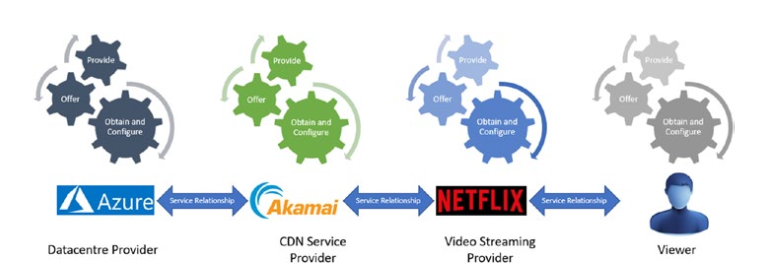
\includegraphics[width=0.8\linewidth]{images/image-03.png}
\end{center}
\end{frame}

\begin{frame}
	\frametitle{Multiple-Choice Question}
	\textbf{Which of these is not an example of a service offering?}
	\begin{enumerate}[A.]
		\item Providing access to service provider’s resources
		\item Goods receivable
		\item Service actions like raising incidents
		\item Amount of money spent on a specific activity
	\end{enumerate}
\end{frame}

\end{document}
